\chapter{实验结果分析}
实验完成了Top-N推荐算法,并对提出的每种推荐算法进行了评估分析,并对实验结果给出了解释。

\section{实验结果度量标准}
推荐系统的度量标准有很多,在我们设计的推荐系统中,我们主要关心推荐出来的商品评分与用户真实的评分之间的误差大小。因此,我们采用较为通用的均方根误差(rmse, root mean square error)方法,其中$r_{pre}$是对一个商品的预测评分,$r_{test}$是对一个商品的真实评分。
\begin{equation}
rmse = \sqrt{\frac{\sum_{i=1}^{n}(r_{pre} - r_{test})^2}{n}}
\end{equation}
在我们的每次实验中,都将输入数据集分割为80\%的训练集和20\%的测试集,使用训练集训练出的模型来对测试集进行预测,并使用rmse公式计算均方根误差。除了我们的实验算法,我们还使用一个用户的平均评分来预测新评分,一个商品的平均评分来预测新评分作为对照组。通过多次实验,我们在后续章节分析实验结果。
\section{ALS算法推荐结果分析}
使用ALS算法,我们需要对算法进行参数训练,寻找到比较好的参数后用于预测。我们的ALS算法接受三个参数,矩阵分解时需要指定的特征数rank值,regParam正则化参数,以及算法的迭代次数iterNum。我们通过对于100k的数据进行参数训练,得到一组较优的参数值,rank=4,regParam=0.1,iterNum=10。我们使用这组参数对后续更大的数据集进行训练。

对于ALS算法的运行结果如图\ref{fig:als}所示,最下面的一条线是使用ALS算法,中间那条是使用itemMean(物品的平均分作为物品的预测得分)的,最上面的线使用的是userMean(用户的平均得分作为用户对一物品的预测得分)。通过图中所示我们可以观察到当数据量增大的时候,rmse基本上与数据量的对数呈现出线性降低关系。随着数据量的增加,使用用户的评分平均分与商品的评分平均分所产生的均方根误差都都在减少,ALS算法的结果明显比其他两类要小。我们还使用0分作为对未知评分的预测,rmse约为3.7。由于与图中的朴素算法相差较大,故没有在图中表现出来。
\begin{figure}[ht]
\centering
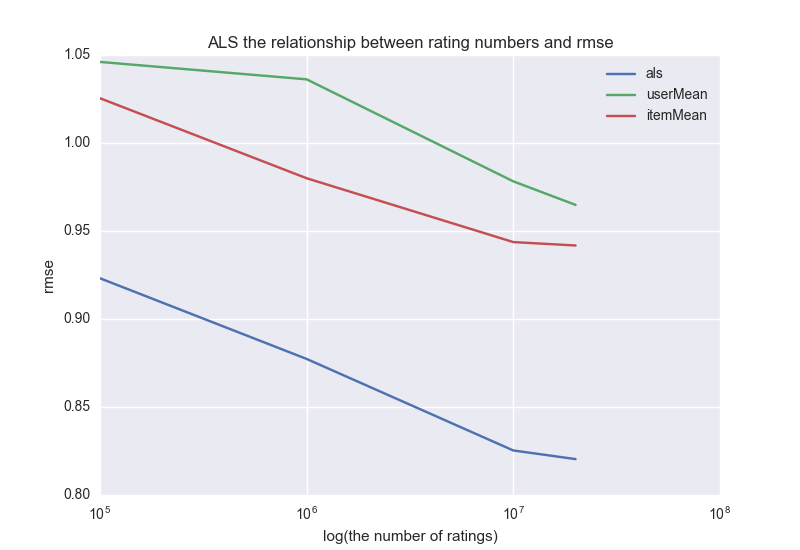
\includegraphics[width=14cm]{als}
\caption{alg}\label{fig:als}
\end{figure}

\section{基于领域关系的算法推荐结果分析}
由于基于邻域的推荐算法对于存储开销要求较大,而我们的集群相对较小,所以在基于邻域的方案中,我们只测试了两组10万数据量的数据集,值得注意的是其中一组为5分制,评价不包含半分,而另一组虽然同样为5分制,但是可以评价半分。我们的计算过程中使用了采样的操作,对于用户-用户的相似关系,限制了用户评价商品的总数,对于商品-商品的相似关系,限制了每个商品所被评价的用户总数。

在图\ref{fig:useruser100k}中,从上到下条线分别采用的是userMean,itemMean和加采样user-user与未加采样的user-user算法。采样总数达到500时基本上基本用户和用户之间的相似关系就已经收敛了,说明这时候已经不需要更多的样本了。在图\ref{fig:itemitem100k}中,从上到下四条线分别为加了采样的item-item,userMean,itemMean,未加采样的item-item算法。此时使用物品-物品的相似性进行推荐,算法最后的收敛效果与朴素的平均值推荐效果类似。由图\ref{fig:useruser100k}和\ref{fig:itemitem100k}中还可以得出另外一个结论,当物品数多于用户数时,我们使用物品的平均分来预测相比使用用户的平均分来预测效果更好一些。
\begin{figure}
\centering
\begin{subfigure}[b]{0.5\textwidth}
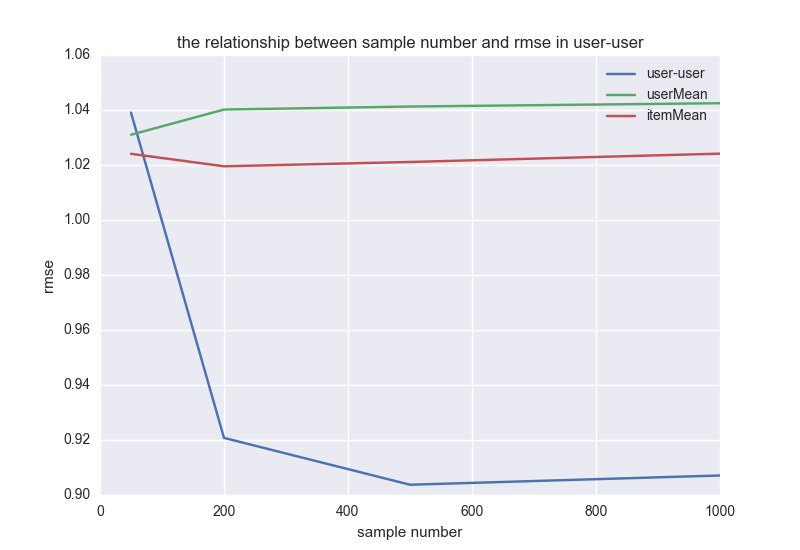
\includegraphics[width=\linewidth]{user-user-100k}
\caption{user\ user\ 100k \ (no half rating)}
\label{fig:useruser100k}
\end{subfigure}%
\hfill
\begin{subfigure}[b]{0.5\textwidth}
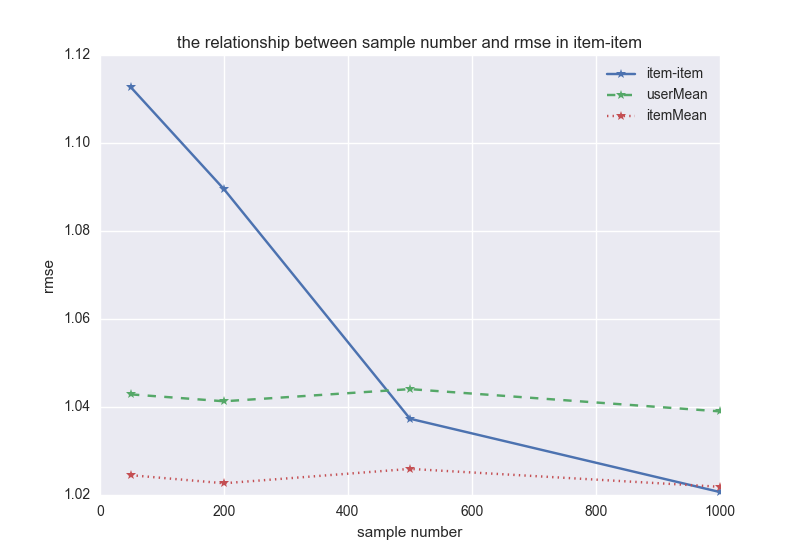
\includegraphics[width=\linewidth]{item-item-100k}
\caption{item\ item\ 100k \ (no half rating)}
\label{fig:itemitem100k}
\end{subfigure}
\caption{不带半分的100K数据分析结果}
\end{figure}

我们在对另外一组使用了包含半分制的评分效果进行分析。在图\ref{userusersmall}中,从上到下四条线分别为itemMean、userMean和加了采样的user-user与未加采样的user-user算法。从图中可以看出,使用user-user算法的推荐结果十分明显优于另外两种对比算法,并且也比在不包含半分的测试中效果要好,在评分包含半分之后,对照组的推荐效果也比上一组实验的对照组要强。这是因为这一组100k的数据中,用户数只有700左右,而商品数达到了10000,所以每个用户的评分数量较多,对于用户的刻画较为准确,而相比之下,每个商品所被评分的用户数就较少,所以基于item-item的评分效果就无基于user-user的评分效果好。
\begin{figure}
\centering
\begin{subfigure}[b]{0.5\textwidth}
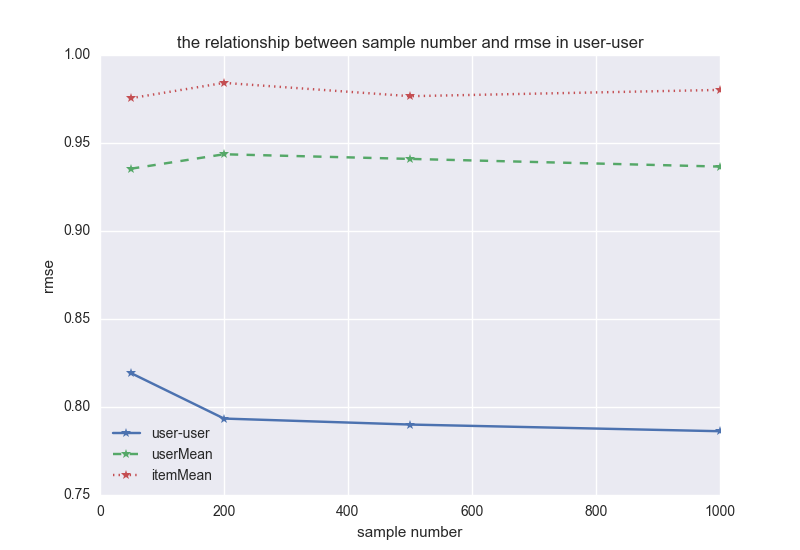
\includegraphics[width=\linewidth]{user-user-small}
\caption{user\ user\ 100k\ (with half rating)}\label{userusersmall}
\end{subfigure}%
\hfill
\begin{subfigure}[b]{0.5\textwidth}
\centering
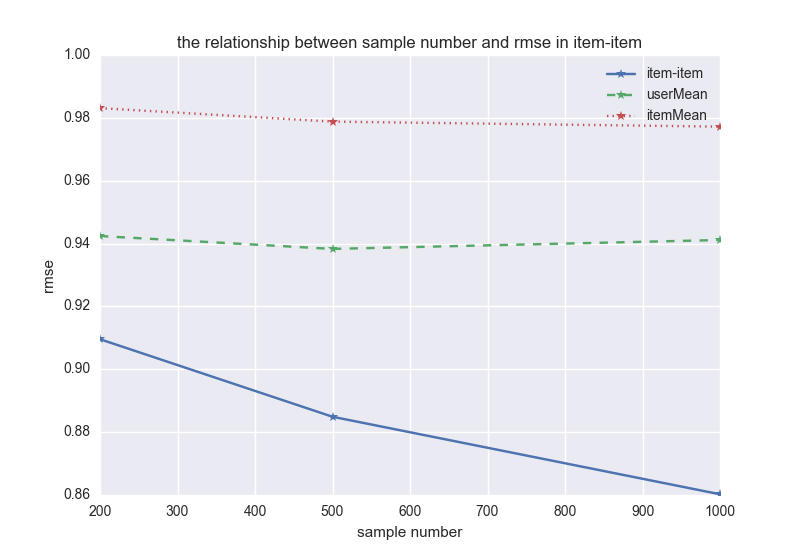
\includegraphics[width=\linewidth]{item-item-small-without-50}
\caption{item item 100k (with half rating)}\label{fig:itemitemsmall}
\end{subfigure}
\caption{带有半分的100K数据数据分析结果}
\end{figure}

我们还对比了一组采样带来的运行时间上的差异,对于带有半分评价的数据集来说,拥有10000的物品,我们对其使用item-item算法得到的运行时间绘图如\ref{fig:runtime}。因为我们在算法中产生item-item对的时候,某些少数活跃的用户可能评分相当之多,影响了整个的运行时间,我们通过对这些用户进行下采样,可以显著提高系统的运行效率。我们需要在对于采样设定的阈值进行权衡,从而可以得到一个较为合理的兼顾计算精度和运行时间的值。

\begin{figure}[ht]
\centering
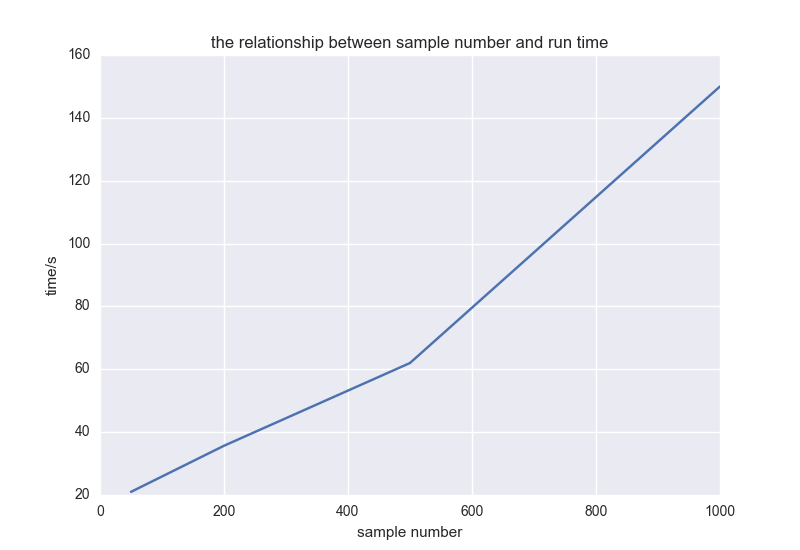
\includegraphics[width=12cm]{runtime}
\caption{runtime}\label{fig:runtime}
\end{figure}

\section{两种算法推荐结果对比总结}
ALS算法随着输入数据的增加,推荐效果越来越好,在数据量较小的时候,推荐效果有时会弱于朴素的推荐算法。基于邻域的推荐算法在数据量较小时就有不错的推荐效果,但是扩展性不如ALS算法,即使我们通过采样的方法使得数据量进行下降,在运算速度上也不如ALS算法,但是基于邻域的推荐算法在推荐算法中是可解释的,我们可以向用户说明,因为和你相似的人也喜欢这个产品,所以我们给你推荐这个产品,或者因为这个产品和你喜欢的某个产品很相似,所以我们给你推荐这个产品,ALS算法计算的结果,我们无法向用户说明推荐的理由。但是因为采用了协同过滤算法中,不包含商品本身的信息,使得我们可能需要计算在真实场景中完全不相关的物品之间的相似性,这可能会导致一定的问题,我们需要根据应用场景来选择所需要的应用算法。
